% This must be in the first 5 lines to tell arXiv to use pdfLaTeX, which is strongly recommended.
\pdfoutput=1
% In particular, the hyperref package requires pdfLaTeX in order to break URLs across lines.

\documentclass[11pt]{article}

% Remove the "review" option to generate the final version.
\usepackage[review]{styles/acl}

% Standard package includes
\usepackage{times}
\usepackage{latexsym}

\usepackage{url}
\usepackage{multirow}
\usepackage{graphicx}
\usepackage{subfigure}
\usepackage{booktabs}
\usepackage{wrapfig}
\usepackage{amsmath}

% For proper rendering and hyphenation of words containing Latin characters (including in bib files)
\usepackage[T1]{fontenc}
% For Vietnamese characters
% \usepackage[T5]{fontenc}
% See https://www.latex-project.org/help/documentation/encguide.pdf for other character sets

% This assumes your files are encoded as UTF8
\usepackage[utf8]{inputenc}

% This is not strictly necessary, and may be commented out,
% but it will improve the layout of the manuscript,
% and will typically save some space.
\usepackage{microtype}


\newcommand{\comment}[1]{{\color{red} #1}}
% If the title and author information does not fit in the area allocated, uncomment the following
%
%\setlength\titlebox{<dim>}
%
% and set <dim> to something 5cm or larger.

\title{Can you ask the question again? Named entity detection via two question-answering-based classifications}

% Author information can be set in various styles:
% For several authors from the same institution:
% \author{Author 1 \and ... \and Author n \\
%         Address line \\ ... \\ Address line}
% if the names do not fit well on one line use
%         Author 1 \\ {\bf Author 2} \\ ... \\ {\bf Author n} \\
% For authors from different institutions:
% \author{Author 1 \\ Address line \\  ... \\ Address line
%         \And  ... \And
%         Author n \\ Address line \\ ... \\ Address line}
% To start a seperate ``row'' of authors use \AND, as in
% \author{Author 1 \\ Address line \\  ... \\ Address line
%         \AND
%         Author 2 \\ Address line \\ ... \\ Address line \And
%         Author 3 \\ Address line \\ ... \\ Address line}

\author{First Author \\
  Affiliation / Address line 1 \\
  Affiliation / Address line 2 \\
  Affiliation / Address line 3 \\
  \texttt{email@domain} \\\And
  Second Author \\
  Affiliation / Address line 1 \\
  Affiliation / Address line 2 \\
  Affiliation / Address line 3 \\
  \texttt{email@domain} \\}

\begin{document}
\maketitle

\begin{abstract}
Named Entity Recognition (NER) is the task of extracting informing entities belonging to predefined semantic classes from raw text. In this paper, we propose to break down the NER task into two logical sub-tasks: (1) Span Detection, which extracts informing entities irrespective of their type and (2) Span Classification, which simply classifies the extracted entities into predefined semantic classes. Both the sub-tasks leverage the full sentence structure and hence do not compromise on any essential information. We demonstrate that this logical separation is (1) effective and (2) time efficient through our experiments on multiple cross-domain datasets using a question-answering framework over the BERT architecture. The effectiveness stems by leveraging the power of the same language model twice, once for each sub-task. This type of modeling allows easy probing to identify performance bottlenecks at sub-task level and deploy personalized models to cater to them.
% (1) how generalizable is this strategy
% (2) BERT model (black box deep model) seems to implicitly decouple the NER task this way
\end{abstract}

\section{Introduction}
\label{sec:intro}
% \comment{
% 1. first paragraph: (1) a couple of sentneces  for NER 
%     and current state of the art; (2)short description on the problem 
%     we try to address in this paper (NER for low resource types)
% 2. a paragraph about our approach: pipeline of span detection and
%     classification. convince the readers
% 3. a short summary on the novelities of the approach and the result
% }

Named Entity Recognition has been %a popular area of Natural Language Processing (NLP) research and serves as 
a foundation step for various applications like question answering, information retrieval and machine translation~\cite{li2020survey}\yjcomment{more citations}. 
Over the years, NER techniques have evolved in sync with new advances in machine learning. 
The advent of the BERT \cite{devlin2019bert} and its effectiveness in capturing text semantics have given new traction to the NER domain. 

For long, NER has been seen as a sequence labeling task where a model is trained to classify each token of a sequence into an output category~\cite{Chiu16,Lample16,ma2016end,devlin2019bert}.
\cite{ma2016end} and \cite{devlin2018bert} show the effectiveness of a CNN-LSTM-CRF and BERT framework for this, respectively. 
In recent years, however, there has been a new trend of formulating NER problems %as question answering(QA) tasks
as span classification tasks\yjcomment{QA based can be viewed as a type of span ner}~\cite{li2020MRC,Jiang20,Ouchi20}, 
where NER is treated as multi-class classification.

Another new trend is formulating NER as a question answering(QA) task~\cite{li2020MRC}. 
Here the model is asked a question as plain text and fed the input sentence. The language model is trained to understand the semantics of the question and identify parts of the input that serve as its answer. \cite{li2020MRC,levy2017zero} model relation extraction as QA tasks and \cite{mccann2018natural} propose a QA-based multi-task learning setup.

However, all of these previous approaches treat the NER problem as a whole. One single model must take a sentence as input and return mention tuples with correct boundaries and correct entity type. 
Further, the existing span classification approaches consider all possible spans up to a predetermined length $l$.
For an input sentence $\{w_1, w_2, \ldots, w_n\}$, these systems enumerate all spans from length 1 to length $l$,
significantly increasing the computation.

We propose a division of labor. We break down the NER problem into a two-step pipelined process. In the first step, \textit{Span Detection}, we detect all mention spans in a given sentence irrespective of their semantic class. In the next step, \textit{Span Classification}, we classify these spans into their corresponding entity type. Using this formulation, we can now train two separate language models independently which specialize in their own sub-tasks and together solve the NER problem. In our experiments, we borrow the basic intuitions of the QA-based NER to solve both our sub-tasks.

Both our sub-task models can be trained independently. The pipeline structure comes during the inference time. Here, every unlabeled sentence is first passed through the \textit{Span Detection} stage and each output span is converted into an input sample for the \textit{Span Classification} stage which assigns each mention span into an entity type thus completing the NER task. We study this proposed logical separation thoroughly by conducting experiments over multiple NER datasets belonging to different domains. Our contributions through this work are:

\begin{itemize}
    \item We demonstrate that our proposed sub-tasks are not tightly coupled to each other and separately handling them does not lead to any degradation in performance compared to modeling the NER task as a whole. 
    
    \item In fact, it helps train a more effective NER system since instead of using the BERT model once for the whole NER task, we are effectively using it twice (fine-tuned for both our sub-task). The similarity of performance in both strategies gives a strong evidence that for NER, the BERT model implicitly does a similar division of labor internally.
    
    \item Training separate models for the sub-tasks gives more flexibility to cater to their respective shortcomings. We propose modeling character patterns for span detection and using dice loss for span classification.
    
    \item We substantiate theoretically and demonstrate experimentally that this logical separation is more efficient and hence takes lesser time to train for equal, if not better performance.
\end{itemize}
\yjcomment{add  (1) unlike other span classification NER, we don't enumerate all potential fixed length spans.  (2) pipeline is more efficient as we can train the two models simultaneously.  (3) more effective as we can better fine-tune the system  optimizing each model (3) more flexible, as we can apply the models indepently. in some cases such as csv or json files,  the mention spans are already known in the input data, so we can only apply the span classification model. }


\section{Pipelined NER}
\label{sec:method}
% - question answering framework is suited to give generalized questions as input and even then expect the model to learn correct answer spans

% - QA effectiveness on identifying accurate entity boundaries (which is key for NER) is already proven by its recent success in NER

% - QA model is found to give high precision/recall for even very generalized entity types (like Genes). This motivates us to gneralize and try bringing all extractable entities under one bucket (motivation for span detection)

% The BERT model is trained on a vast English corpus and the deeply interconnected transformer architecture ensures that the so-called foundational model learns some generalized semantics and language attributes which can be fine-tuned and reoriented to suit for a variety of NLP tasks, one such being NER.

% In the NLP domain, there are several standardized problem settings or paradigms, like sequence labeling, sentence classification. An NLP application can be approached (or solved) through several of these problem settings. For example, one way of looking at NER task is through sequence labeling where each token of a sequence is to be labeled into an output class, like \texttt{Person}, \texttt{Organization}. The NER task has been traditionally looked at from this perspective. However, recently the question-answering setting has gained popularity for NER, where a question is fed as plain text, like, "Where is the Person mentioned in the text?" along with the sentence input and a model is trained to output the right span where the entity in question is present. \cite{} show the effectiveness of the question-answering paradigm for NER over the BERT architecture. Here on, we refer to this as the \texttt{BERT-QA} setup. We implemented the \texttt{BERT-QA} setup, trained it on multiple datasets (OntoNotes, BioNLP13CG, WNUT) and qualitatively studied the model outputs to draw two broad findings:

% \begin{enumerate}
%     \item \textbf{Finding 1}: Entity mentions belonging to the same entity type can occur in different parts of the sentence depending on sentence style.
    
%     \item \textbf{Finding 2}: Entity mentions belonging to different entity types can occur in similar parts of the sentence.
% \end{enumerate}

% The findings are substantiated through examples in Table \ref{tab:ner_problem_ex}. Based on the findings, we can conclude that identifying entity mentions and inferring their entity types can be decoupled and treated as separate tasks. This gives the advantage that entity mention extraction rules can be shared across entity types and in case of datasets with high class imbalance, the rare entities can benefit from rules derived from mentions of the frequent ones. 

% This motivates us to break down the NER task into two sub-tasks, \textit{Span Detection} and \textit{Span Classification}, each of which are trained independent of each other. \textit{Span Detection} is entity-type agnostic and forms generalized rules to identify mention spans. The \textit{Span Classification} stage takes these mention span outputs from the previous stage and associates them with their entity types.

% In fact, through the similarity of our results as shown later in the paper, an NER system performing well on a dataset which does not violate the findings stated above, inherently is performing the span detection and classification tasks separately. 

In our system, the NER task is performed by a combination of two separately trained modules -- \textit{Span Detection Module}
and \textit{Span Classification Module}.
The first one, \textit{Span Detection Module}, identifies all mention spans by learning entity-agnostic rules for extraction. This helps the low-resource entity types (with very few mentions) borrow knowledge from the high-resource entity types (which have a rich diversity of mention samples in training data). 
% Note that our span detection setup is formulated as a simpler NER task, where there are only 4 target labels (BIEO).
% Our method is completely different from other span classification-based methods~\cite{li2020MRC,Jiang20,Ouchi20}, which consider all possible spans up a predetermined length in a input sequence. 
All these extracted mention spans are fed as input to the second module, \textit{Span Classification Module}, which reanalyses them in the sentence structure and looks at how they interact with the other entities of the sentence to classify it into a target entity type. In this way, both the modules, even though being separate from each other, have complete access to full sentence structure and do not suffer from lack of any essential information for their sub-tasks.
%\yjcomment{be more specific instead of `essential information'}.

This separation gives us the freedom to train both modules independently (can be done in parallel) and optimized and fine-tuned for their intended sub-tasks. Even if done sequentially, these sub-tasks are much simpler than the generalized NER task and as we show later, give a significant efficiency boost with no compromise in performance.

We adopt the BERT-QA framework as the underlying architecture of both the models, but
use different features and loss functions. \comment{check if required and add a bit more about the architecture and add the overall system diagram here}

\begin{figure*}
    \centering
    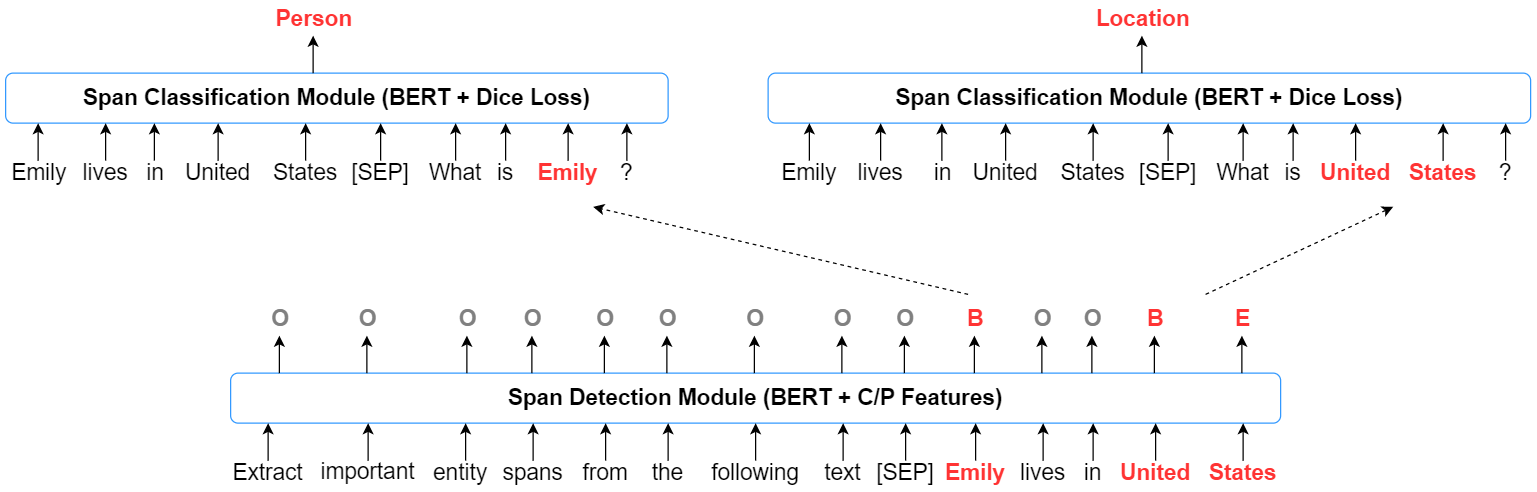
\includegraphics[width=\linewidth]{framework5.png}
    \caption{Span Detection Setup with \texttt{BIOE} scheme and \textit{What is the entity mentioned in the text?} as the question (colored tokens depict the generic entity type in question and gold entity mentions with expected output labels}
    \label{fig:framework}
\end{figure*}

\subsection{Features}
\label{sec:features}
\comment{explain the features we use}


\subsection{Span Detection}
\label{sec:span}
Given a sentence $\mathcal{S}$ as a $N$-length sequence of tokens, $\mathcal{S} = \langle w_1, w_2 \ldots w_N \rangle$, the goal of this module is to output a list of spans (mention tuples) $\langle s, e\rangle$ where $s \in [1, N]$ is the \textit{start} index, $e \in [1, N]$ is the \textit{end} index. Note that here the mention tuples are not associated with an entity type. 

We formulate this as a question answering task asking the model to identify all entity spans in a given sentence. For example, the sentence, \textit{Emily}[\texttt{PERSON}] \textit{lives in United States}[\texttt{LOCATION}], is converted to the input, \textit{What is the \texttt{entity} mentioned in the text? Emily lives in United States}. This is fed to BERT model which outputs labels for each token following the \texttt{BIOE} scheme. In this example, we expect two spans, \textit{Emily} and \textit{United States}. Figure \ref{fig:span_detection} shows our span detection setup.

\begin{figure}
    \centering
    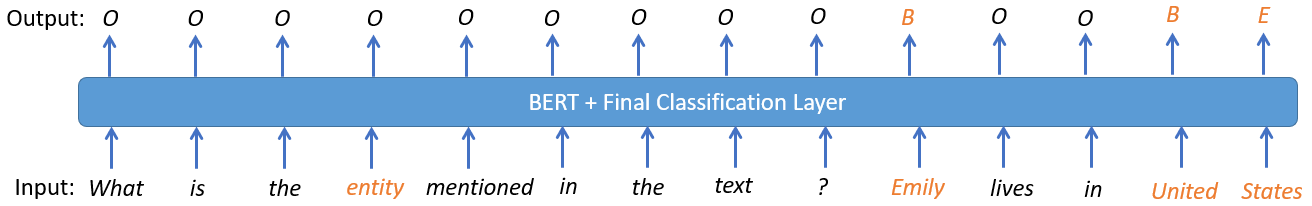
\includegraphics[width=\linewidth]{../thesis/span_detection}
    \caption{Span Detection Setup with \texttt{BIOE} scheme and \textit{What} as question word (colored tokens depict the generic entity type in question and gold entity mentions with expected output labels)}
    \label{fig:span_detection}
\end{figure}



\subsection{Span Classification}
\label{sec:class}
Here, we are given a sentence $\mathcal{S}$ as a $N$-length sequence of tokens, $\mathcal{S} = \langle w_1, w_2 \ldots w_N \rangle$ and a span $\langle s, e\rangle$ where $s \in [1, N]$ is the \textit{start} index, $e \in [1, N]$ is the \textit{end} index. The goal is to output a label $t$ for the span such that $t \in \mathcal{T}$, where $\mathcal{T}$ is the set of all entity types.

This is modeled as the reverse of QA model for NER described in Section \ref{sec:span}. For every gold entity mention (E.g. \textit{United States}) in a training set sentence, \textit{Emily}[\texttt{PERSON}] \textit{lives in United States}[\texttt{LOCATION}], we form a sample input, \textit{Emily lives in United States. What is United States?} The sentence is fed to a BERT model where we do sequence classification. The pooled sequence embedding returned by BERT is fed to a fully connected layer and converted to a probability distribution over possible entity types. In this example, the model is expected to assign maximum probability to \texttt{LOCATION}. Figure \ref{fig:span_classification} shows our span classification setup.

\begin{figure}[h!]
    \centering
    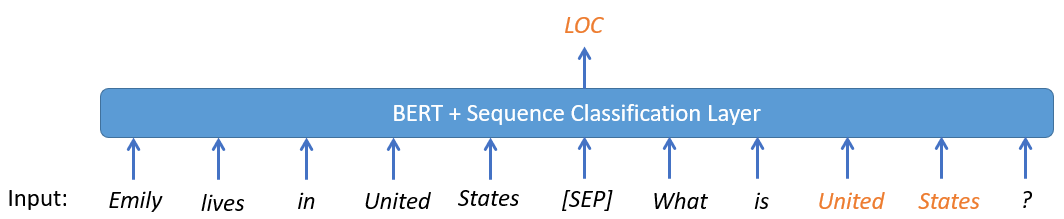
\includegraphics[width=\linewidth]{resources/span_classification}
    \caption{Span Classification Setup (colored tokens depict the entity mention in question with expected output entity label)}
    \label{fig:span_classification}
\end{figure}

- is reverse question answering setup
- is a simpler step in general compared to span detection. 
- may suffer from biases because of lots of classes and class imbalance. 
- Dice loss has been shown to be effective. So, we adopt it here as well.
- Later ablations show its effectiveness

\subsection{Learning Objective Function}
\label{sec:loss}
As detailed earlier, Cross Entropy is an accuracy-oriented objective while during evaluation, we calculate the F1-Score. This difference can lead to sub-optimal model training. To counteract, \cite{li2019dice} make use of S{\o}rensen-Dice coefficient(DSC)\cite{sorensen1948method, dice1945measures} and Tversky index\cite{tversky1977features} which are F-Score oriented statistics. Given sets $A$ and $B$, DSC is used to gauge similarity among two sets and is defined as,
\begin{equation}
\label{eq:dsc_set}
    DSC(A, B) = \frac{2\ \vert A \cap B \vert}{\vert A \vert + \vert B \vert}
\end{equation}
Consider $A$ as set of all positive samples predicted by a model and $B$ as set of all ground truth positives. Then, by definition of true positive ($TP$), false positive ($FP$) and false negative ($FN$) from Section \ref{sec:evaluation_metrics}, we have,
\begin{equation}
\label{eq:dsc_tp}
    TP = \vert A \cap B \vert
\end{equation}
\begin{equation}
\label{eq:dsc_a}
    \vert A \vert = TP + FP
\end{equation}'
\begin{equation}
\label{eq:dsc_b}
    \vert B \vert = TP + FN
\end{equation}
Using Equations \ref{eq:dsc_tp}, \ref{eq:dsc_a} and \ref{eq:dsc_b}, in Equation \ref{eq:dsc_set}, we get,
\begin{equation}
\label{eq:dsc_as_f1}
     DSC(A, B) = \frac{2TP}{2TP + FP + FN} = \frac{2\ \frac{TP}{TP + FN}\ \frac{TP}{TP + FP}}{\frac{TP}{TP + FN} + \frac{TP}{TP + FP}} = \frac{2\ Precision \times Recall}{Precision + Recall} = F1
\end{equation}

The dice coefficient gives equal importance to false-positives and false-negatives at training time and is more immune to data-imbalance issues\cite{sudre2017generalised, shen2018influence, kodym2018segmentation}. The above formulation (Equation \ref{eq:dsc_as_f1}) shows its equivalence to F1-score thus removing the discrepancy among training and evaluation metrics. From Equation \ref{eq:dsc_set}, for an individual sample $x_i$, dice coefficient is defined as,
\begin{equation}
\label{eq:dsc_per_sample}
    DSC(x_i) = \frac{2p_{i1}y_{i1} + \gamma}{p_{i1} + y_{i1} + \gamma}
\end{equation}
where $\gamma$ is the smoothing parameter. Then over all samples, from Equation \ref{eq:dsc_per_sample}, dice loss (DL) is defined in Equation \ref{eq:dice_loss} as:
\begin{equation}
\label{eq:dice_loss}
    DL = 1 - \frac{2\sum_i{p_{i1}y_{i1}} + \gamma}{\sum_i{p_{i1}} + \sum_i{y_{i1}} + \gamma}
\end{equation}


\section{Experimental Results}
\label{sec:exp}
We have conducted extensive experiments to validate 
the effectiveness of our pipeline approach for NER tasks. 

\subsection{Data}
We validate our system using four datasets belonging to the general, biomedical and cybersecurity domains.
We use \data{OntoNotes5.0} and \data{WNUT17} for the general domain and \data{BioNLP13CG} for the biomedical domain, 
which are all publicly available.
For the cybersecurity domain, we use a private dataset, 
which contains news articles, blogs and technical reports related to malware, hacking groups and vulnerabilities.
We denote the dataset as \data{CyberThreats} in this paper.

We note that these datasets can demonstrate the effectiveness of our algorithms especially for non-word, low-resource (i.e., small number of training instances) entity types using the datasets from multiple domains and noisy text.
The datasets include not only traditional entity types with word mentions(e.g., PERSON, LOCATION) but also many entity types with non-word (Antivirus Signature) and very long mentions (e.g., URL, Software with version, etc).
Table \ref{tab:datasets_summary} shows a summary of the datasets.
\begin{table*}[h!]
\centering
\begin{small}
\begin{tabular}{ccccrrr}\toprule
 \textbf{Dataset} & \header{\#Entities} & \header{Non-Word} & \header{Low Resource} & \header{Train} & \header{Dev.} & \header{Test} \\ \toprule 
\data{BioNLP13CG} & 16 & Yes & Yes & 3,033  & 1,003 & 1,906 \\
\data{CyberThreats} & 8 & Yes & Yes & 38,721 & 6,322 & 9,837 \\
\data{OntoNotes5.0} & 18 & Yes & Yes & 115,812 & 15,680 & 12,217 \\  
\data{WNUT17} & 6 & Yes & Yes & 3,394 & 1,287 & 1,009\\
\bottomrule
\end{tabular}
\caption{Overview of the experimental datasets. \header{\#Entities} indicates the number of unique entity types.
\header{Non-Word} and \header{Low Resource} indicate if the dataset contains non-word mentions (e.g, mentions with digits and symbols) and low-resource entity types respectively.  
\header{Train}, \header{Dev.} and \header{Test} show the number of sentences in the datasets.}
\label{tab:datasets_summary}
\end{small}
\end{table*}

\yjcomment{Shall we show the class distribution for the datasets? We need to use the names of diffrent methods consistently. Let's make a name for our system instead of Span-Pipeline.}
\comment{Different domains (entity nature \& language context) / dataset sizes / No. of entities 
- BIONLP13CG: Bio dataset (using Scibert + BERT model)
- OntoNotes: General entities / newswire (using Roberta base)
- WNUT17: emerging entities from tweets (using BERT)
Also show from result analysis that span class is simpler and gives above 90\% result where as detector is the main bottleneck}

%%%%%%%%%%%%%%%%%%%%%%%%%%%%%%%%%%%%%%%%%%%%%%%%%

\subsection{Experimental Setup}
We use \deptool{transformers}\footnote{https://github.com/huggingface/transformers} library from \deptool{HuggingFace} and \deptool{pytorch} for implementation. 
For general English corpora like \data{OntoNotes5.0} and \data{WNUT17}
and the cybersecurity data, we use a pretrained BERT model (bert-base-uncased\footnote{https://huggingface.co/bert-base-uncased}). 
For the biomedical dataset (\data{BioNLP13CG}), we use SciBERT
(scibert\_scivocab\_uncased\footnote{https://github.com/allenai/scibert}), a language model for scientific text~\cite{beltagy-etal-2019-scibert}. 

Note that. in all our experiments, we only use the BERT-Base architecture, which has around 110 million trainable parameters. 
The training data is randomly shuffled and a batch size of $16$ is used with post-padding. We fixed random seed to $42$ for replication.
For BERT-based models, we set the maximum sequence length to $256$ for \data{BioNLP13CG}, \data{CyberThreats} , and \data{WNUT17} and to $512$ for \data{OntoNotes5.0}. 


We use the cross entropy loss during training unless otherwise specified. 
The development set evaluation takes place at steps of 0.5 training epochs. We train the models for $300$ epochs at learning rate $10^{-5}$ unless otherwise specified.
The BERT-based models output entity labels for each sub-token (as per WordPiece tokenization) of an existing token in the dataset. 
We take the label of the first sub-token as the label for the corresponding token for the evaluations.
We use Nvidia GeForce GTX 1080 and Nvidia Tesla V100 GPUs for model training and evaluation.

%%%%%%%%%%%%%%%%%%%%%%%%%%%%%%%%%%%%%%%%%%%%%%%%%

\subsection{Baseline Systems}
\yjcomment{Jatin -- please update this section}


We present this comparison since QA model serves as the primary backbone of our span-based approach. 
All models here use BIOE tagging scheme.
For span detection, we use \textit{Extract important entity spans from the following text} as the question irrespective of the entity types.
For span classification, we use \textit{What is $<mention>$} where $<mention>$ is the string value for an extracted span by the span detection model.  

\if false  
\texttt{BERT}: Proposed by \cite{devlin2018bert}, BERT is a bidirectional encoder transformer\cite{vaswani2017attention}. It applies WordPiece\cite{wu2016google} tokenization on input sentence which is then passed through several encoder layers with multiple attention heads capturing sentence semantics and inter-token relationships well. The model outputs contextualized embeddings for each sub-token in the sentence. We take the last hidden layer outputs from BERT model and pass it to a fully connected layer. The outputs are converted to a probability distribution over labels space. Model parameters are initialized from a pretrained model and fine-tuned on our NER task.


\texttt{BERT-Freeze}: To understand how much semantic information is already captured in a pretrained BERT model, we use the exact same architecture as \texttt{BERT} model above but freeze the BERT model parameters. So, the only trainable parameters remain from the fully connected layer. For this setting, we use learning rate as $0.005$.

\texttt{CNN-LSTM-CRF}: \comment{better to include this as a baseline since it is very widely used}
\fi

\subsection{Performance Comparison}
We compare the performances of our system, the baseline systems and the best reported 
state-of-the-art (SOTA) tools. 
All of our models' results were measured on the test sets using the model checkpoint corresponding to the best Micro F1-score on the development sets. 
Table~\ref{tab:res_span} shows the comparison results based on the mention-level Micro F1 scores on the test sets (i.e., only the exact matches are considered correct).
\begin{table*}[h!]
\centering
\begin{small}
\begin{tabular}{ccccc}\toprule
 \textbf{Model} & \texttt{BioNLP13CG} & \texttt{CyberThreats} & \texttt{OntoNotes} & \texttt{WNUT17} \\ \toprule 
BERT-QA & 86.69 & \textcolor{blue}{ongoing(y1)} & \textcolor{blue}{ongoing(j)}  & 44.60 \\
BERT-Span-Pipeline-Vanilla     & 86.69 & \textcolor{red}{todo} & 90.12 & 55.36  \\
BERT-Span-Pipeline     & 86.70 & \textcolor{red}{todo} & 90.31 & 56.30  \\
Reported SOTA & 85.56(thesis see) & N/A & 92.07(MRC-Dice) & 60.45(CL-KL)  \\
\bottomrule
\end{tabular}
\caption{Comparison of the NER results on the four datasets. The numbers indicate the mention-level Micro F1 scores. 
\yjcomment{can you find the results of SOTA without any external data or additional pretraining? I consider MRC-Dice also using additional info. as they added several synonyms/hyponyms in query.   we can put SOTA without external data and with external data in separate rows if you like. We point out that our system does not rely on external knowledge which is usually unavailable for domain-specific data and needs less computing resources than MRC}}
\label{tab:main}
\end{small}
\end{table*}

\paragraph{Feature Analysis}
To investigate the effectiveness of the character sequence and pattern embeddings,
we performed the span detection tasks with and without the character and pattern features.
In Table~\ref{tab:det_ablation}, we report the mention-level precision (P), recall (R) and F1 scores
by the two models. 
As we can from the results, adding pattern and character features improve the precision while
maintaining similar recall levels.
\begin{table*}[h!]
\centering
\begin{small}
\begin{tabular}{ccccccccccccc}\toprule
 \multirow{2}{*}{\textbf{Model}} & \multicolumn{3}{c}{\data{BioNLP13CG}} & \multicolumn{3}{c}{\data{CyberThreats}} & \multicolumn{3}{c}{\data{OntoNotes5.0}} & \multicolumn{3}{c}{\data{WNUT17}} \\ \cmidrule{2-12} 
 & P & R & F1 & P & R & F1 & P & R & F1 & P & R & F1 \\ \midrule
Char-Pattern & 91.43 & 90.70 & 91.06 & & & 78.63 \textcolor{blue}{ongoing(y4)}& & & 92.50 & & & 55.21  \\
No Char-Pattern& & & 90.67 &79.65 & 77.77 & 78.70 & & & 92.37 & 72.63 & 44.06 &54.85  \\
\bottomrule
\end{tabular}
\caption{Performance comparison of span detection with and without character and pattern embeddings}
\label{tab:det_ablation}
\end{small}
\end{table*}


\paragraph{Loss Function}
A recent study has shown that using dice coefficient as the loss function was more beneficial than 
the cross entropy loss for NLP tasks with imbalanced data~\cite{li2019dice}. 
Inspired by this work, we trained our span classification model, which has the data imbalance problem,
using both cross entropy loss and dice loss.
Our experiments also confirm that the dice loss provides a small improvement over the cross entropy loss 
as shown in Table~\ref{tab:class_ablation}.
\begin{table*}[h!]
\centering
\begin{small}
\begin{tabular}{ccccc}\toprule
 \textbf{Model} & \texttt{BioNLP13CG} & \texttt{CyberThreats} & \texttt{OntoNotes} & \texttt{WNUT17} \\ \toprule 
Span-Classification-Dice & 94.27 & 87.84 &  96.74 & 73.40  \\
Span-Class-CE     & 94.04 & 87.58 & 96.50 & 73.31  \\
\bottomrule
\end{tabular}
\caption{Span Classification Results with different loss functions}
\label{tab:class_ablation}
\end{small}
\end{table*}

\paragraph{Training Time}
As discussed in Section~\ref{sec:method}, our pipeline approach applying span detection  and span classification separately is more efficient than combined models.
To validate the assertion, we measured the training times of our pipeline system
and the baseline BERT-QA, which uses exactly the same features and underlying architecture but performs span detection and classification in one unified model.
All experiments were done using two V100 GPUs with 16G memory on each GPU. 
The results confirm that the pipeline approach is much more efficient,
and, the efficiency improvement grows as the size of training data and 
the number of entity types grow.
\begin{table*}[h!]
\centering
\begin{small}
\begin{tabular}{ccccc}\toprule
 \textbf{Model} & \texttt{BioNLP13CG} & \texttt{CyberThreats(10\%)} & \texttt{OntoNotes(10\%)} & \texttt{WNUT17} \\ \toprule 
BERT-QA                & 1,372.8 & 877.1 &  7,381.8   & 568.2\\
Span-Pipeline     & 241.2 (106.3/134.9) & 145.53 (113.7/31.9) & 300.8 (185.5/115.3)  & 122.9 (98.9/24.0)\\
\bottomrule
\end{tabular}
\caption{Comparison of the training time between our method and a non-pipeline QA-based NER method. 
    The training time is reported in seconds per training epoch. The numbers in the parentheses denote the training times for span detection and span classification respectively. }
\label{tab:train_time_ablation}
\end{small}
\end{table*}

\begin{table*}[h!]
\centering
\begin{small}
\begin{tabular}{cccccc}\toprule
      &  \textbf{} & BioNLP13CG & JNLPBA & CoNLL2003 & OntoNotes5.0\\\toprule
\multirow{3}{*}{Baseline} & \texttt{BERT-Freeze} &  75.42 & 55.93 & 82.79 & 67.35 \\
                          & \texttt{BERT} & 85.99 & 74.35 & 91.36 & 83.39 \\ 
                          & \texttt{BERT-QA} & \textbf{86.45} & 74.81 & 91.17 & \\\midrule
\multirow{3}{*}{OurModel} &        \texttt{Span Detection} & 90.12 & 78.35 & 95.23 & \\
        & \texttt{Span Classification} & 94.06 & 95.08 & 94.50 & \\
        & \texttt{Pipeline} & 85.89 & \textbf{75.01} & \textbf{91.64} & \\ \bottomrule
\end{tabular}
\caption{The classificaiton results of our system and the state of the art method over 4 benchmark datasets. 
     The numbers reprent the Micro-F1 in \% on the test datasets.}
    \label{tab:res_span}
\end{small}
\end{table*}

%\comment{need more results and some plots}

\if false
Next, we deep dive into the \texttt{BioNLP13CG} dataset which has $16$ entity types including several high and low-resource types. We compare the model performance at the entity type level for our 3 major NER approaches: sequence labeling, question answering and span-based pipeline. We compare our best performing model variants through entity-level and macro-averaged F1-scores. Let $\mathcal{T}$ be the set of all entity types and F1$_t$ be the F1-score for individual entity type $t \in \mathcal{T}$. Then, Macro-averaged F1-Score is defined in Equation \ref{eq:macro_f1} as:
\begin{equation}
\label{eq:macro_f1}
    \text{Macro-F1} = \frac{1}{\mathcal{\vert\mathcal{T}\vert}}\,\sum_{t\,\in\,\mathcal{T}}{\text{F1}_t}
\end{equation}
We present the comparison among the following models:
\begin{itemize}
    \item \texttt{Dice Loss}: Sequence labeling NER approach over BERT model with \texttt{BIO} tagging scheme and dice loss instead of cross entropy.

    \item \texttt{Special Symbol}: Sequence labeling NER approach over BERT with \texttt{BIO} tagging scheme and additional one-hot input feature to capture if a token is a special symbol like \textit{hyphen}, or \textit{parenthesis}.

    \item \texttt{BERT-QA (Where)}: Question answering NER approach with \texttt{BIOE} tagging scheme and \textit{Where} as the question word.

    \item \texttt{Span Based}: Pipelined approach which uses the QA setup with \texttt{BIOE} tagging scheme and \textit{What} as question word for span detection and QA-based sequence classification for span classification.
\end{itemize}

\begin{figure}
    \centering
    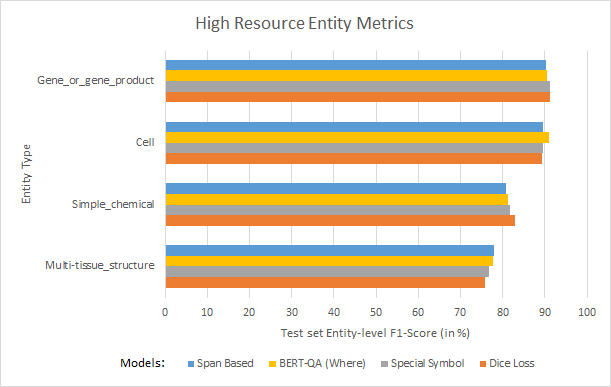
\includegraphics[scale=0.5]{../thesis/high_resource_entity_metrics}
    \caption{Test set Entity-level F1 scores for high resource entities in \texttt{BioNLP13CG} dataset}
    \label{fig:high_resource_entity_metrics}
\end{figure}

\begin{figure}
    \centering
    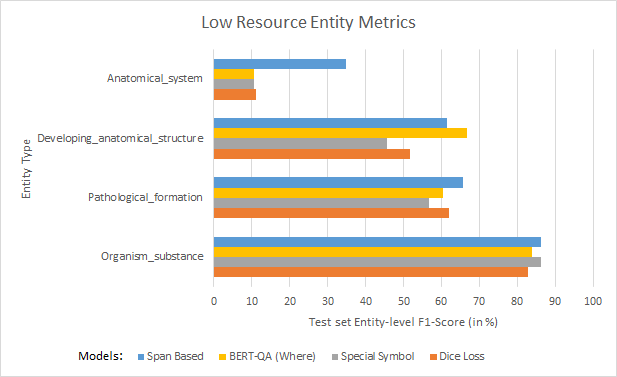
\includegraphics[scale=0.5]{../thesis/low_resource_entity_metrics}
    \caption{Test set Entity-level F1 scores for low resource entities in \texttt{BioNLP13CG} dataset}
    \label{fig:low_resource_entity_metrics}
\end{figure}

\fi


\section{Discussions}
\label{sec:discussion}
From the results of experiments reported in the previous section, we make the following observations:

\begin{itemize}
    \item From Table \ref{tab:main}, we see that \modelname{} outperforms sequence tagging and QA-based baselines on three cross-domain datasets and performs on-par with the baseline on \data{BioNLP13CG} demonstrating the effectiveness of our proposed division of labor. 
    
    \item The results show that span detection and classification tasks have minimal correlation with each other and can be done independent of each other. 
    
    \item Compared to the baseline approaches, \modelname{} has more representative power. This is because we have two BERT models (rather than one) each working on their own sub-tasks and contributing towards better NER. % while the baselines just have a single model.
    
    \item Comparison with baselines gives some additional insights into the internal functioning of BERT model which also implicitly tries to learn entity-agnostic extraction rules for mentions. Our approach explicitly models this behavior and hence is found to be more effective.
    
    \item \data{WNUT17} has a diverse range of rare and emerging entities crudely categorized into $6$ entity types. A single-model NER system may get confused and try to learn sub-optimal entity-specific extraction rules. Our task segregation allows \spandetect{} to form generalized extraction rules which is found to be more effective as shown in Table \ref{tab:main}.
    
    \item As a sidenote, all our baselines and \modelname{} outperform the previously published approaches on \data{BioNLP13CG} (Table \ref{tab:main}), thus setting new state-of-the-art results. However, the credit here goes to the SciBERT model, 
    better training parameters and the added character and pattern features.
    
    \item \modelname{} leverages the QA framework much more efficiently than the standard single-model NER systems (Table \ref{tab:train_time_ablation}). The margin of improvement is more pronounced with the increase in data size and number of entity types.
    
    \item Table \ref{tab:train_time_ablation} considers the components of \modelname{} being trained sequentially. However, the approach is flexible enough to train both models in parallel, reducing the train time even further. The sequential nature is necessary only at inference time.
    
    % \item Comparing the F1 scores in Table \ref{tab:det_ablation} and Table \ref{tab:class_ablation}, detecting correct mention spans is harder than disambiguating them and classifying them into entity types. However, both the sub-tasks are simpler than the overall NER task.
    
    \item From results in Table \ref{tab:det_ablation}, adding character and pattern features indeed helps detect better boundaries improving precision while maintaining recall thus giving better F1 score in \spandetect{}.
    
    \item Further, Table \ref{tab:feature_ablation} shows that adding character and pattern features independently helps span detection. The effect is more pronounced when both are added together. However, adding POS features does not help, indicating that POS semantics is well captured by existing BERT features and the added character and pattern features.
    
    \item Table \ref{tab:class_ablation} shows that dice loss helps handle the class imbalance issues seen in \spanclass{} and gives a slight performance improvement over cross entropy loss.
\end{itemize}

\subsection{Qualitative Analysis}
Table \ref{tab:quality} shows some sample predictions by \modelname{} and compares them  with \method{BERT-QA}. Note that \method{BERT-QA} is a standard single-model NER system and does not use our proposed character and pattern features or dice loss. We observe that,
\begin{itemize}
    \item \modelname{} is better in detecting emerging entities and out-of-vocabulary (OOV) terms (for example, movie titles and softwares) which may be rare and have high diversity. This can be attributed to \spandetect{} being stronger in generalizing and sharing entity extraction rules across multiple entity types.
    
    \item \method{BERT-QA} gets confused when entities have special symbols within them (for example, hyphens and commas). Our character and pattern features in \spandetect{} help handle such cases well.
    
    \item \method{BERT-QA} model develops a bias towards more common entity types like \type{Location} and misclassifies rare entity mentions (like \type{Product}) when they occur in a similar context. \modelname{} handles such cases well with the help of a dedicated \spanclass{} using dice loss.
\end{itemize}

\begin{table}
\centering
\begin{small}
\begin{tabular}{cl}\toprule
 Category &  {~~~~~~~~~~~~}Example Sentence \\\toprule
\multirow{2}{*}{\shortstack{General \\ Detection}}     
     & CVS selling their own version of ... \\
     & \textit{\textcolor{red}{CVS}} selling their own version of ... \\ \midrule
\multirow{2}{*}{\shortstack{Emerging \\ Entities}}  
    &Rogue One create a plot hole in Return of the Jedi ...  \\
     & \textit{\textcolor{Turquoise}{Rogue One}} create a plot hole in \textit{\textcolor{Turquoise}{Return of the Jedi}} ...  \\ \midrule
\multirow{2}{*}{\shortstack{Scientific \\ Terms}} 
     & Treating EU - 6 with anti-survivin antisense ...  \\
     & Treating \textit{\textcolor{brown}{EU - 6}} with anti-survivin antisense ... \\ \midrule
\multirow{2}{*}{Boundary}  
   & .. Hotel Housekeepers Needed in Spring , \textit{\textcolor{ForestGreen}{TX}} ...  \\
    & .. Hotel Housekeepers Needed in \textit{\textcolor{ForestGreen}{Spring , TX}} ...  \\ \midrule
\multirow{2}{*}{\shortstack{OOV \\ Terms}}  
   & Store SQL database credentials in a webserver \\
    & Store \textit{\textcolor{magenta}{SQL}} database credentials in a webserver \\ \midrule
 \multirow{2}{*}{\shortstack{Entity \\ Type}}  
  & Why do so many kids in \textit{\textcolor{ForestGreen}{Digimon}} wear gloves? \\
    & Why do so many kids in \textit{\textcolor{magenta}{Digimon}} wear gloves? \\ \bottomrule
\end{tabular}
\caption{Qualitative comparison of \modelname{} and \method{BERT-QA} systems. For each category, the first line shows the result of \method{BERT-QA},
and the second line shows the result of \modelname{}. 
% The words in italics are the entity mentions extracted by the systems, and red, blue, brown, green, and magenta colors denote \type{Org}, \type{Creative Work}, \type{Gene},  \type{Location} and \type{Product}  types respectively.
The words in italics are the entity mentions extracted by the systems color-coded as \textcolor{red}{\type{Org}}, \textcolor{Turquoise}{\type{Creative Work}}, \textcolor{brown}{\type{Gene}}, \textcolor{ForestGreen}{\type{Location}} and \textcolor{magenta}{\type{Product}}
}
    \label{tab:quality}
\end{small}
\end{table}

%%%%%%%%%%%%%%%%%%%%%%%%%%%%%%%% old version
\if false
\begin{table*}[h!]
\centering
\begin{small}
\begin{tabular}{ccc}\toprule
Category & Model & Example \\\toprule
\multirow{2}{*}{General Detection} & \bertqa{} & \textit{CVS selling their own version of ...} \\
    & \modelname{} & \textit{\textcolor{blue}{CVS}[\texttt{Corporation}] selling their own version of ...} \\ \midrule
\multirow{2}{*}{Emerging Entities} & \bertqa{} & \textit{Does Rogue One create a plot hole in Return of the Jedi ... } \\
    & \modelname{} & \textit{Does \textcolor{blue}{Rogue One}[\texttt{Creative Work}] create a plot hole in \textcolor{blue}{Return of the Jedi}[\texttt{Creative Work}] ... } \\ \midrule
\multirow{2}{*}{Scientific Terms} & \bertqa{} & \textit{The MVD and Ki - 67 LI were higher ... } \\
    & \modelname{} & \textit{The MVD and \textcolor{blue}{Ki - 67}[\texttt{Gene}] LI were higher ...} \\ \midrule
\multirow{2}{*}{Boundaries} & \bertqa{} & \textit{.. Hotel Housekeepers Needed in Spring , \textcolor{blue}{TX}[\texttt{Location}] ... } \\
    & \modelname{} & \textit{.. Hotel Housekeepers Needed in \textcolor{blue}{Spring , TX}[\texttt{Location}] ... } \\ \midrule
\multirow{2}{*}{Out of Vocab Terms} & \bertqa{} & \textit{Store SQL database credentials in a webserver} \\
    & \modelname{} & \textit{Store \textcolor{blue}{SQL}[\texttt{Product}] database credentials in a webserver} \\ \midrule
\multirow{2}{*}{Entity Classification} & \bertqa{} & \textit{Why do so many kids in \textcolor{blue}{Digimon}[\texttt{Location}] wear gloves?} \\
    & \modelname{} & \textit{Why do so many kids in \textcolor{blue}{Digimon}[\texttt{Product}] wear gloves?} \\ \bottomrule
\end{tabular}
\caption{Examples from multiple datasets comparing performance of \modelname{} and \bertqa{} systems}
    \label{tab:quality}
\end{small}
\end{table*}


\begin{table}[h!]
\centering
\begin{small}
\begin{tabular}{p{0.5in}p{0.5in}p{2in}}\toprule
 Category & Model & Example \\\toprule
\multirow{2}{*}{\shortstack{General \\ Detection}} &     
    \method{BERT-QA} & \textit{CVS selling their own version of ...} \\
    & \modelname{} & \textit{\textcolor{blue}{CVS}[\type{ORG}] selling their own version...} \\ \midrule
\multirow{2}{*}{\shortstack{Emerging \\ Entities}} & 
  \method{BERT-QA} & \textit{Does Rogue One create a plot hole in Return of the Jedi ... } \\
     &  \modelname{} & \textit{Does \textcolor{blue}{Rogue One}[\type{Creative Work}] create a plot hole in \textcolor{blue}{Return of the Jedi}[\type{Creative Work}] ... } \\ \midrule
\multirow{2}{*}{\shortstack{Scientific \\ Terms}} & 
    \method{BERT-QA} & \textit{The MVD and Ki - 67 LI were higher ... } \\
     & \modelname{} & \textit{The MVD and \textcolor{blue}{Ki - 67}[\type{Gene}] LI were higher ...} \\ \midrule
\multirow{2}{*}{Boundary} & 
  \method{BERT-QA} & \textit{.. Hotel Housekeepers Needed in Spring , \textcolor{blue}{TX}[\type{Location}] ... } \\
    & \modelname{} & \textit{.. Hotel Housekeepers Needed in \textcolor{blue}{Spring , TX}[\type{Location}] ... } \\ \midrule
\multirow{2}{*}{\shortstack{OOV \\ Terms}} & 
   \method{BERT-QA} & \textit{Store SQL database credentials in a webserver} \\
    & \modelname{} & \textit{Store \textcolor{blue}{SQL}[\type{Product}] database credentials in a webserver} \\ \midrule
 \multirow{2}{*}{\shortstack{Entity \\ Type}} & 
  \method{BERT-QA} & \textit{Why do so many kids in \textcolor{blue}{Digimon}[\type{Location}] wear gloves?} \\
    &  \modelname{} & \textit{Why do so many kids in \textcolor{blue}{Digimon}[\type{Product}] wear gloves?} \\ \bottomrule
\end{tabular}
\caption{Examples from multiple datasets comparing performance of the \modelname{} and \bertqa{} systems. \method{BERT-QA} refers \bertqa{} in this table.}
    \label{tab:quality}
\end{small}
\end{table}

\fi
%%%%%%%%%%%%%%%%%%%%%%%%%%%%%%%% old version

\section{Related Work}
\label{sec:related}
NER has been a popular research topic in the field of natural language processing for long. The progress can be categorized into four classes namely, rule-based/dictionary-based techniques\cite{quimbaya2016named}, unsupervised methods\cite{zhang2013unsupervised}, feature-engineering approaches\cite{mcnamee2002entity} and more recently deep learning-based approaches\cite{torfi2020natural, li2020survey}. Our focus here is more on the recent deep learning methods. \cite{devlin2018bert, peters2018deep, akbik2018contextual} propose contextualized word/string representations to better model sentence semantics thus improving NER performance. Deep learning systems are however limited by the amount of labeled training data. Hence, there have been efforts to generate noisy labeled data as weak supervision signals for training. \cite{shang2018learning} propose AutoNER framework which uses distant supervision for generating noisy labels for training. \cite{arora2017extracting} use regular expression patterns for artificial training data generation and train a LSTM model for entity extraction. \cite{zhou2019dual} propose adversarial perturbations and use CNN-LSTM-CRF architecture to train a robust model with limited gold data. \cite{liu2018empower, liu2018efficient} train a task-aware language model from unlabeled data which guides NER. As a side note, sometimes gold labels in datasets may have some errors. \cite{wang2019crossweigh} use a bootstrapping framework to correct such imperfect annotations.

In scientific and biomedical domain, NER has its own set of challenges. Entity mentions are long and may have alpha-numeric symbols, chemical formulas etc. which may be hard for a language model to make sense of. Many entity types also low-resource with a shortage of labelled training data. \cite{wang2019cross} use a multi-task learning framework and combine labelled data from multiple corpora mapping entity tags across corpora to coherent classes. \cite{wang2020pattern} use noisy distant supervision from domain-specific dictionaries. \cite{wang2018penner} form entity-type meta patterns for entity extraction. \cite{wang2019distantly} make use of a setup similar to AutoNER\cite{shang2018learning} tailor-made for biomedical NER. \cite{wang2020fine, wang2020comprehensive} apply weak or distant supervision for NER on COVID-19 literature.

Several named entities have numeric nature, for example, phone numbers and SSNs look very much alike and require understanding of number patterns to differentiate the two. NER systems deadling with such entities need some explicit numeral semantic handling. \cite{chen2019numeracy} propose a Bi-GRU framework for understanding numbers. \cite{wallace2019nlp} shows that standard contextual word embeddings like ELMo\cite{peters2018deep}, BERT\cite{devlin2018bert} have some good sense of numbers and character-level embeddings are more effective than word-level embeddings in capturing numeral semantics.


\section{Conclusion}
Taking inspiration from the QA setup, we proposed the span detection and classification pipeline which uses a reverse question formulation. We also proposed to convert from a sparse character space to a dense pattern space through which we can learn meaningful intrinsic character patterns in alphanumeric and pattern-oriented entities. We demonstrated the effectiveness of our proposed domain-agnostic techniques on multiple datasets in general English and biomedical domains. 
%We also presented a study depicting that trivial concatenation of external semantic vectors with BERT outputs may not train the model effectively at lower learning rates.

Our span-based setup opens up prospects for more intuitive and creative ways of approaching the NER problem. However, the pipelined nature of the approach currently serves as a bottleneck. It may be worthwhile to think of some ensemble-based approach where we train individual BERT models on some sub-problems and each of those models contributed its part to solve the overall NER problem in a majority-voting setup.

%Our study on training effectiveness reveals that feeding additional external semantics while fine-tuning the BERT model is non-trivial. This again motivates future research on designing feature fusion techniques which are effective with a BERT (transformer-like) architecture.

From the qualitative analysis of the various approaches, we observe that boundary detection serves as a primary issue in NER. To alleviate this problem, we explicitly model word types and special symbols. However, there is still a wide margin to cover. We encourage the research community to design architectures or new training objectives tailor-made to handle mention boundaries effectively. 


%\section*{Acknowledgements}

% Entries for the entire Anthology, followed by custom entries
\bibliographystyle{styles/acl_natbib}
\bibliography{thesisrefs.bib}
%\bibliography{anthology,custom}

%\appendix

%\section{Example Appendix}
%\label{sec:appendix}


\end{document}
